\section{Qualitative Analysis and Manual Audit}
\label{sec:qualitative}
Every row below is drawn by a seeded random choice inside a rule-defined stratum, and \ours{}' \emph{failures} are
shown as often as its successes. Each row shows the crop, the
ground truth, the claim, PARSeq's reading, \ours{}' probability and whether its decision is right (red: wrong), the
repair proposal for rejected incorrect claims, and the evidence of the three strongest rivals relative to the claim,
$\Delta\rho_V(v)=\rho_V(v)-\rho_V(h)$, for TrOCR (blue) and PARSeq (orange); a positive bar means that verifier finds the
rival a better explanation of the image than the claim, and $*$ marks the ground truth.

\begin{figure}[t]\centering
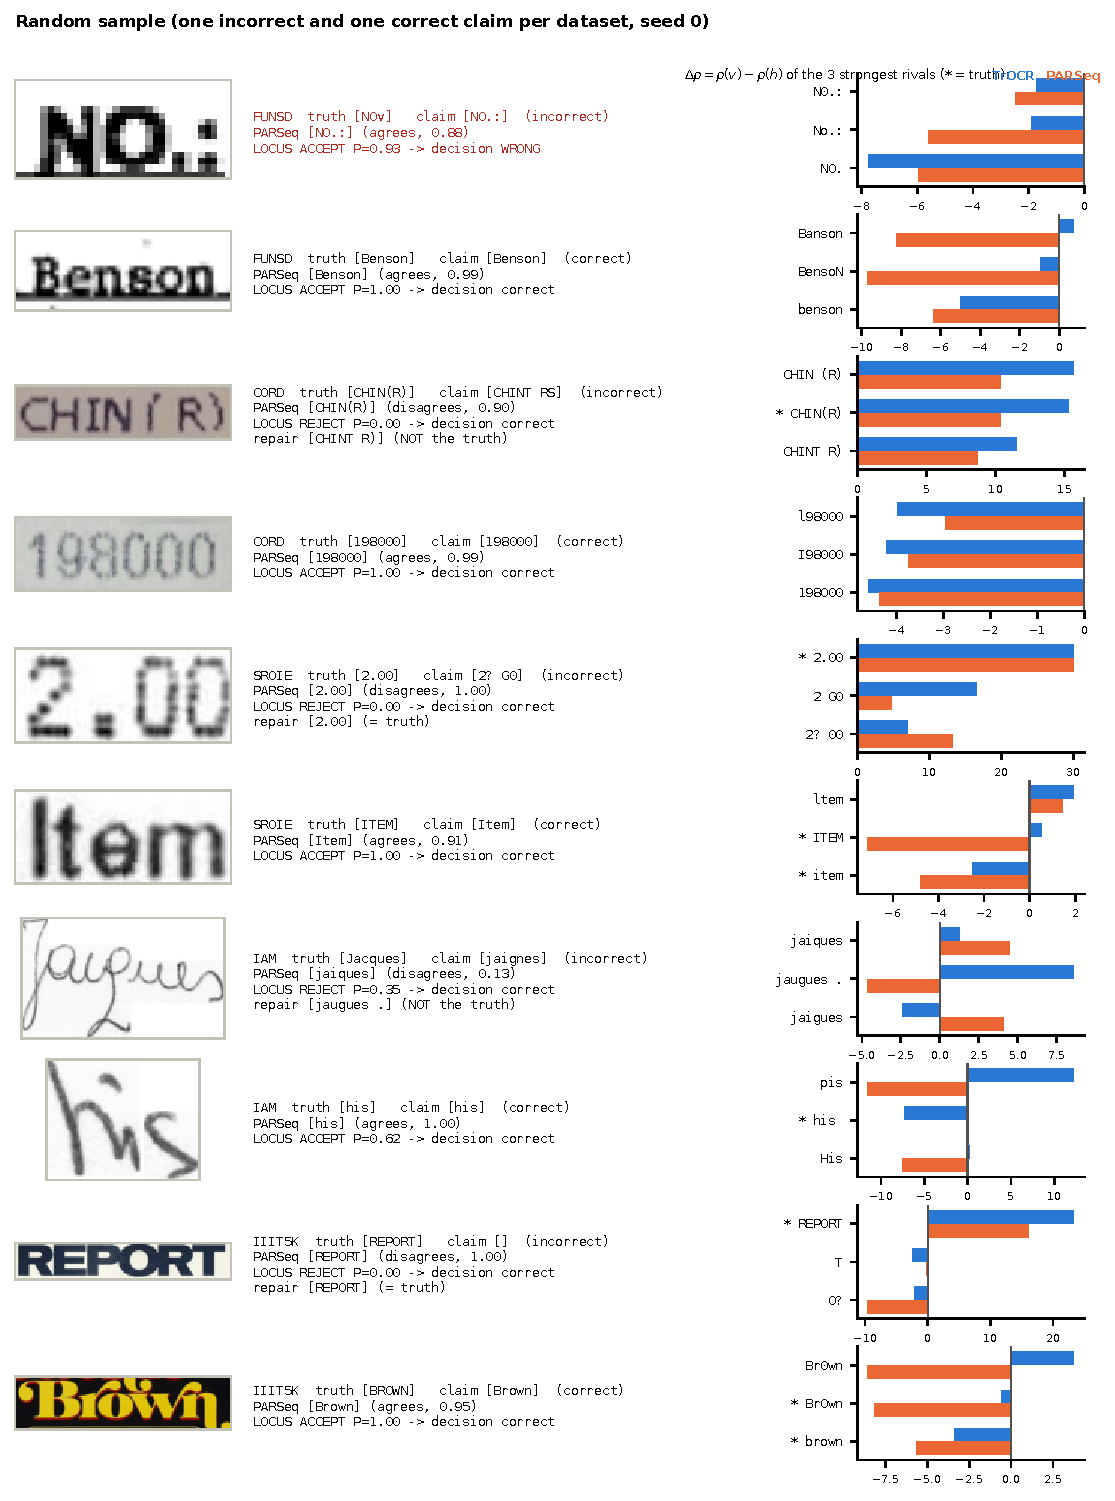
\includegraphics[width=0.74\linewidth]{figs/qual_random.pdf}
\caption{\textbf{Random sample} (seed 0): one incorrect and one correct claim per dataset, drawn without regard to
\ours{}' output; wrong decisions in red. Annotation errors also appear (e.g.\ FUNSD ground truth ``NOv'' for a crop
reading ``NO.:''; Table~\ref{tab:audit}).}
\label{fig:qual_random}
\end{figure}

\begin{figure}[t]\centering
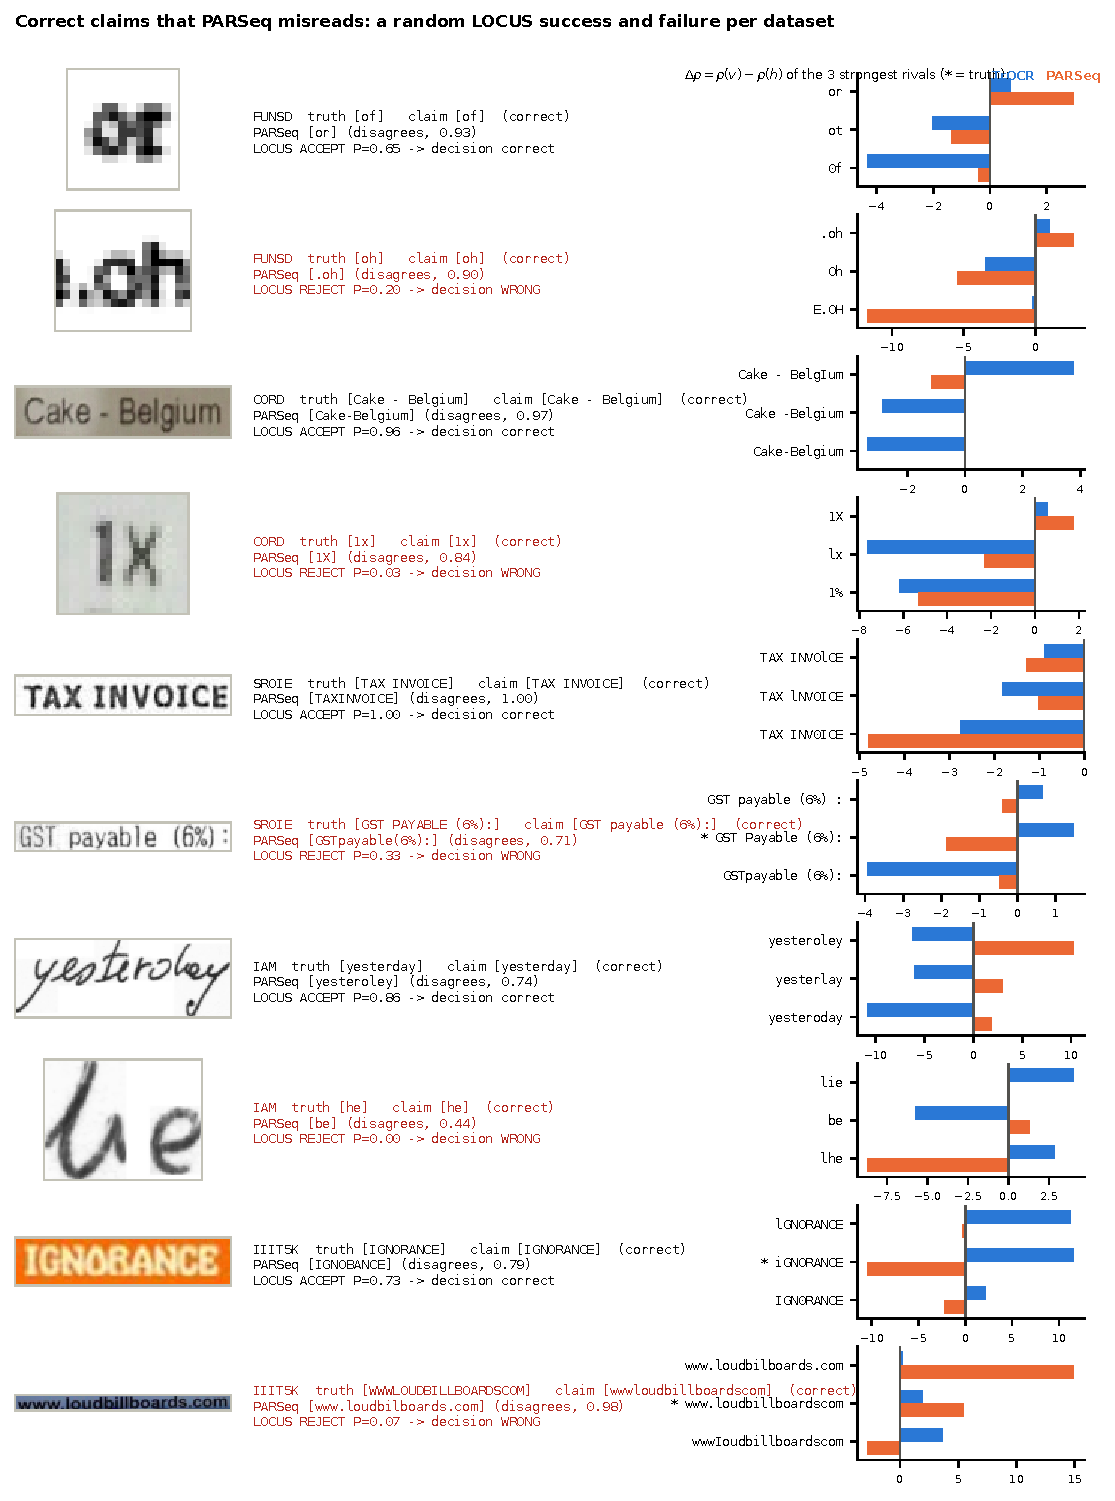
\includegraphics[width=0.74\linewidth]{figs/qual_regime_misread.pdf}
\caption{\textbf{Correct claims that PARSeq misreads} (re-recognition would reject them): one random \ours{} success and
one random failure per dataset. Comparing the claim with its rivals under two verifiers helps most in this regime: a
rival that one verifier prefers is typically rejected by the other.}
\label{fig:qual_misread}
\end{figure}

\textbf{Regimes.} Table~\ref{tab:qual_counts} counts the two regimes that matter on the full test sets. Correct claims
that PARSeq misreads are frequent on every dataset, and \ours{} accepts most of them (Figure~\ref{fig:qual_misread}); this
is the regime in which comparing hypotheses under two verifiers pays off. Character errors that PARSeq reproduces are
rarer and \ours{} rejects only a small fraction of them (Supplementary Figure~\sref{fig:qual_fooled}).

\begin{table}[t]\centering
\caption{\textbf{Regimes on the full test sets} ($k=25$). Artefacts: incorrect claims that differ from the ground truth
only in case or punctuation. Right: errors PARSeq agrees with, restricted to genuine character errors.}
\label{tab:qual_counts}
\footnotesize\setlength{\tabcolsep}{3pt}\resizebox{\linewidth}{!}{\begin{tabular}{lcccccc}\toprule
& \multicolumn{2}{c}{all errors} & \multicolumn{2}{c}{correct claims PARSeq misreads} & \multicolumn{2}{c}{character errors PARSeq agrees with}\\
Dataset & count & artefacts & count & \ours{} accepts & count & \ours{} rejects\\\midrule
\tabinput{tables/qual_counts.tex}
\bottomrule\end{tabular}}\end{table}

\textbf{Manual audit.} To understand the errors behind these numbers, we inspected two random samples of up to 20 test
words per dataset: (i) words on which \ours{} decides wrongly and (ii) incorrect claims that PARSeq agrees with. Each crop
was labelled \emph{genuine} (the ground truth matches the visible text), \emph{label noise}, \emph{crop problem} (text
clipped or a neighbouring glyph inside the box) or \emph{ambiguous} (Table~\ref{tab:audit}). \AUDITSENTENCE{} The audit
was performed by a single annotator; the annotated sheets are released with the code.

\begin{table}[t]\centering
\caption{\textbf{Manual audit} of random test words (20 per cell, fewer where the stratum is smaller). G: genuine, N:
label noise, C: crop problem, A: ambiguous, P: claim correct only under the dataset's normalisation protocol although
its exact appearance differs from the image (IIIT5K only).}
\label{tab:audit}
\footnotesize\begin{tabular}{lccccccccc}\toprule
& \multicolumn{5}{c}{\ours{} decision wrong} & \multicolumn{4}{c}{errors PARSeq agrees with}\\
Dataset & G & N & C & A & P & G & N & C & A\\\midrule
\tabinput{tables/audit.tex}
\bottomrule\end{tabular}\end{table}
